% docs/texte/20_core/spectral_lines.tex -- chapter "Spectral Lines" (Interferosim)
% Version: 0.1.0 (2026-11-01) -- spectra, Doppler correction, multichannel visibilities (interferosim 0.9.0)
% ================================================================
\label{ch:spectral-lines}
\index{spectral line}\index{LSR}\index{Doppler correction}\index{OH maser}\index{HI absorption}

Continuum and line spectra of the sky components, the Doppler correction to
the local standard of rest and multichannel visibilities. Implemented in
version~0.9.0; notebook \texttt{09\_spectral\_lines.ipynb}.

\section{Implementation}

\begin{description}
  \item[\texttt{sky.spectra}] the spectrum gives the shape of a component
        over frequency, $S(f) = S_0\,\mathrm{shape}(f)$:
        \texttt{FlatSpectrum}, \texttt{PowerLawSpectrum} ($(f/f_\mathrm{ref})^\alpha$),
        \texttt{GaussianLineSpectrum} (Gaussian line in velocity, $S_0$ = peak),
        \texttt{AbsorptionSpectrum} (power-law continuum times $e^{-\tau(v)}$,
        $\tau$ a sum of Gaussians). Velocities in the radio convention
        $v = c\,(f_0-f)/f_0$. In the JSON sky model a component carries the key
        \texttt{"spectrum"}; \texttt{SkyModel.spectra} holds them by component
        name, components without a spectrum stay flat.
        \texttt{SkyModel.flux\_at}, \texttt{at\_frequency} (continuum snapshot for
        all single-frequency tools), \texttt{spectrum\_jy},
        \texttt{visibility\_spectrum}.
  \item[\texttt{observation.doppler}] velocity of the observer relative to
        the LSR from the Earth's rotation, the orbit (derivative of the
        low-precision solar position referred to J2000) and the standard solar
        motion (20\,km/s towards RA $18^\mathrm{h}03^\mathrm{m}50.29^\mathrm{s}$,
        Dec $+30^\circ00'16.8''$); $v_\mathrm{LSR} = v_\mathrm{topo} +
        \vec v_\mathrm{obs}\cdot\hat s$ (\texttt{v\_lsr\_correction\_kms});
        agreement with astropy (barycentric correction plus the same solar
        motion) within 0.02\,km/s. \texttt{topocentric\_frequency\_hz} sets the
        LO, \texttt{regrid\_to\_lsr} interpolates every row of a fixed-LO
        recording onto a common LSR velocity axis (Doppler tracking in
        software).
  \item[\texttt{SpectralVisibilitySimulator}] $N$ channels of width
        $\Delta f = B/N$ (layout of the FX correlator), LO fixed at the
        frequency of a chosen LSR velocity at transit; every channel at its own
        spatial frequency and with the component spectra, converted to the LSR
        frame per integration; noise per channel
        $\sqrt{(\mathrm{SEFD}_i+S_i(f))(\mathrm{SEFD}_j+S_j(f))/(2\Delta f\,t)}$.
  \item[\texttt{Imager.channel\_images}] one dirty image per channel (image
        cube).
\end{description}
New sky models: \texttt{w3oh\_masers\_lines} (the maser group with
1665\,MHz lines of 0.4\,km/s at $-44.0$, $-45.8$ and $-42.3$\,km/s) and
\texttt{cyg\_a\_hi} (Cygnus~A, $\alpha = -0.7$, HI absorption $\tau = 0.6$ at
$+3$\,km/s and 0.3 at $-80$\,km/s); the velocities and optical depths are
illustrative values, not catalogue data.

\section{Results}

\paragraph*{Doppler correction.} For W3(OH) the correction varies by
$\pm0.25$\,km/s within a day and by tens of km/s over the year
(Fig.~\ref{fig:lines-lsr}); on 2026-11-01 it is $+10.8$\,km/s, and the
maser at $-44$\,km/s is received 61\,kHz above its LSR frequency.

\begin{figure}[htbp]
  \centering
  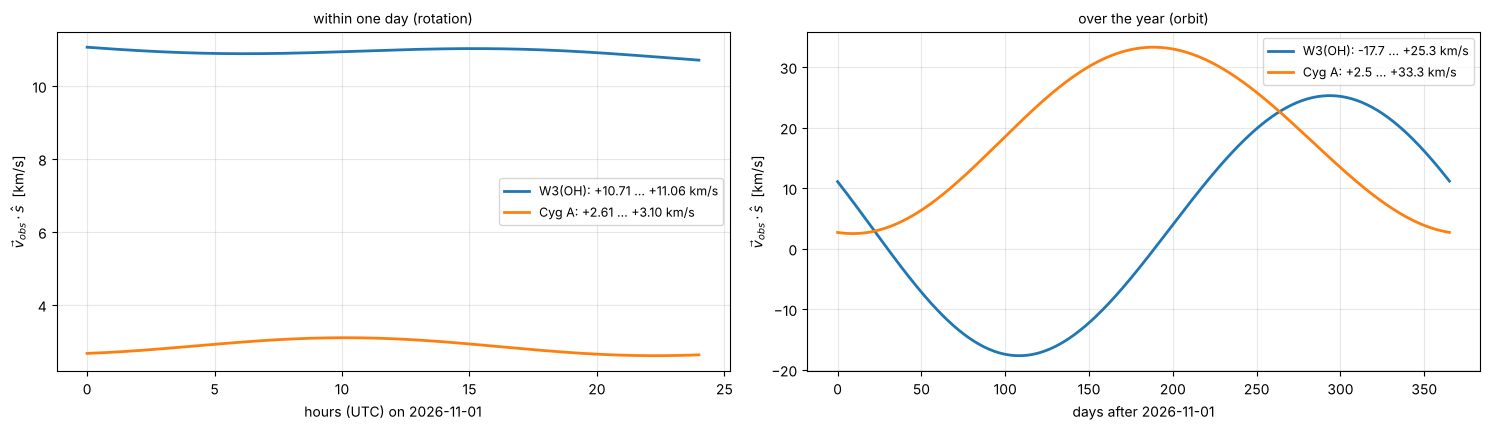
\includegraphics[width=\textwidth]{images/lines_lsr.png}
  \caption{LSR correction $\vec v_\mathrm{obs}\cdot\hat s$ for W3(OH) and
           Cygnus~A at Wilhelmsburg: within one day and over one year.}
  \label{fig:lines-lsr}
\end{figure}

\paragraph*{OH masers on the 11.5\,km baseline.} 125\,kHz in 128 channels
(0.18\,km/s), $\pm8$\,h, two 3\,m dishes: noise 228\,Jy per visibility and
channel, 7.4\,Jy after 16\,h. The lines drift through the topocentric channels
with the Earth's rotation; after regridding to the LSR the spectrum towards
each maser position (phase centre shifted, vector average) shows M1 and M2
clearly, M3 (17.5\,Jy in its channel, $2.4\sigma$) is lost in the noise
(Fig.~\ref{fig:lines-masers}). In the channel maps each maser is alone; the
average of all channels dilutes the narrow lines by about 1/50 and loses them
(Fig.~\ref{fig:lines-maps}). Without the Doppler correction the M1 line
appears at $-54.8$ instead of $-44.0$\,km/s.

\begin{figure}[htbp]
  \centering
  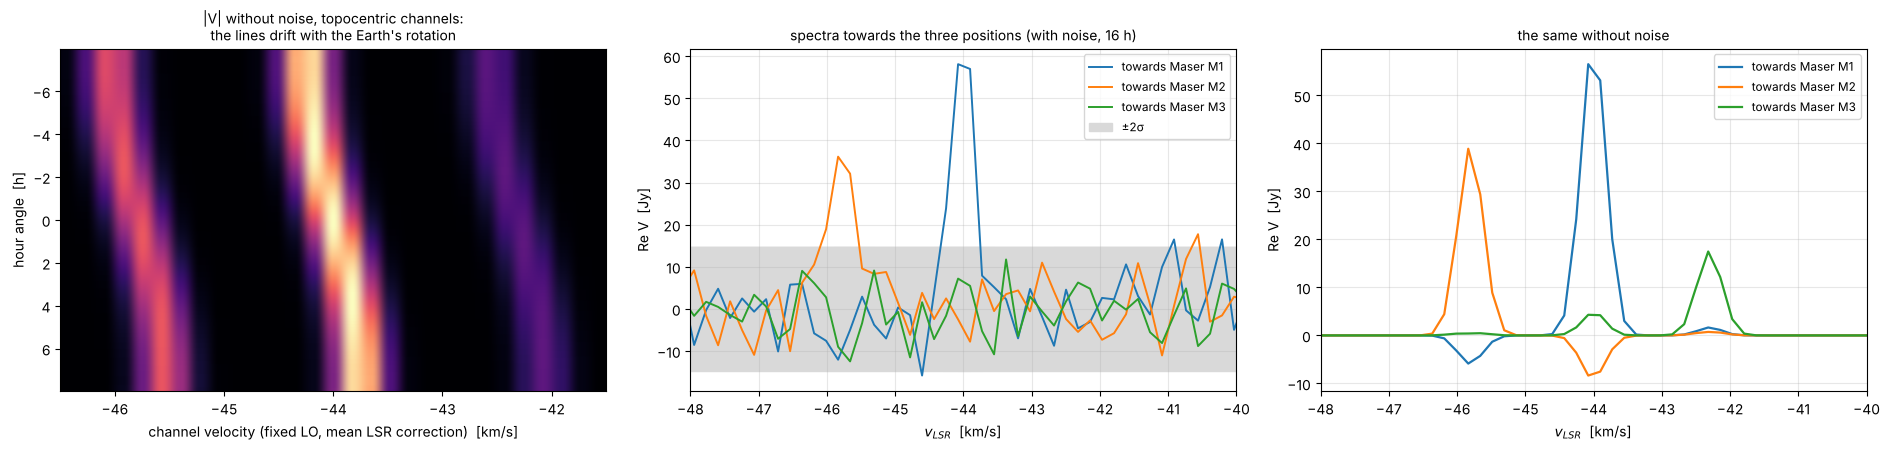
\includegraphics[width=\textwidth]{images/lines_masers_spectra.png}
  \caption{Maser group on the 11.5\,km baseline: noise-free amplitude over
           hour angle and topocentric channel (drift), spectra towards the three
           maser positions after regridding, with noise and without.}
  \label{fig:lines-masers}
\end{figure}

\begin{figure}[htbp]
  \centering
  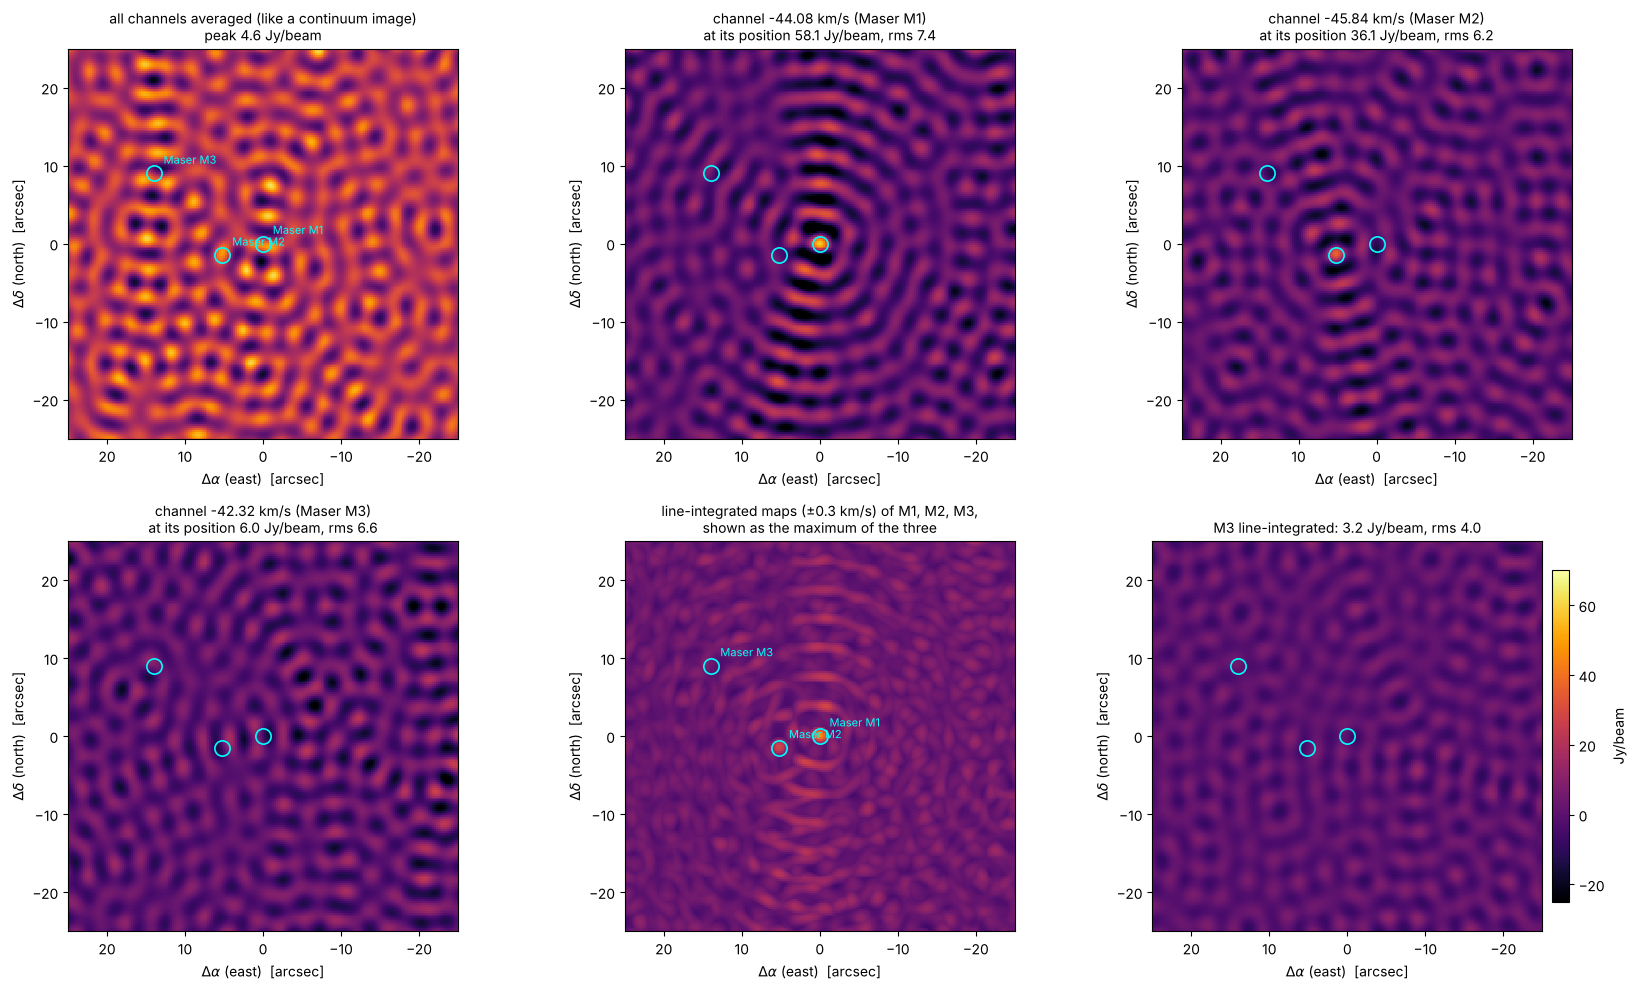
\includegraphics[width=\textwidth]{images/lines_channel_maps.png}
  \caption{Average of all channels, the channels of the three maser velocities,
           and line-integrated maps ($\pm0.3$\,km/s).}
  \label{fig:lines-maps}
\end{figure}

\paragraph*{HI absorption against Cygnus~A.} 1\,MHz in 128 channels
(1.65\,km/s). The absorption multiplies every visibility, so the ratio
$\hat R(v) = \sum_r V_r(v)V^*_{r,\mathrm{cont}}/\sum_r|V_{r,\mathrm{cont}}|^2$
gives $e^{-\tau}$ even on baselines that see only the hotspots: $\tau = 0.60$
and 0.34 (true 0.59 and 0.30) with an rms of 0.049 in the line-free channels on
the project baseline, 0.020 with three stations
(Fig.~\ref{fig:lines-hi}).

\begin{figure}[htbp]
  \centering
  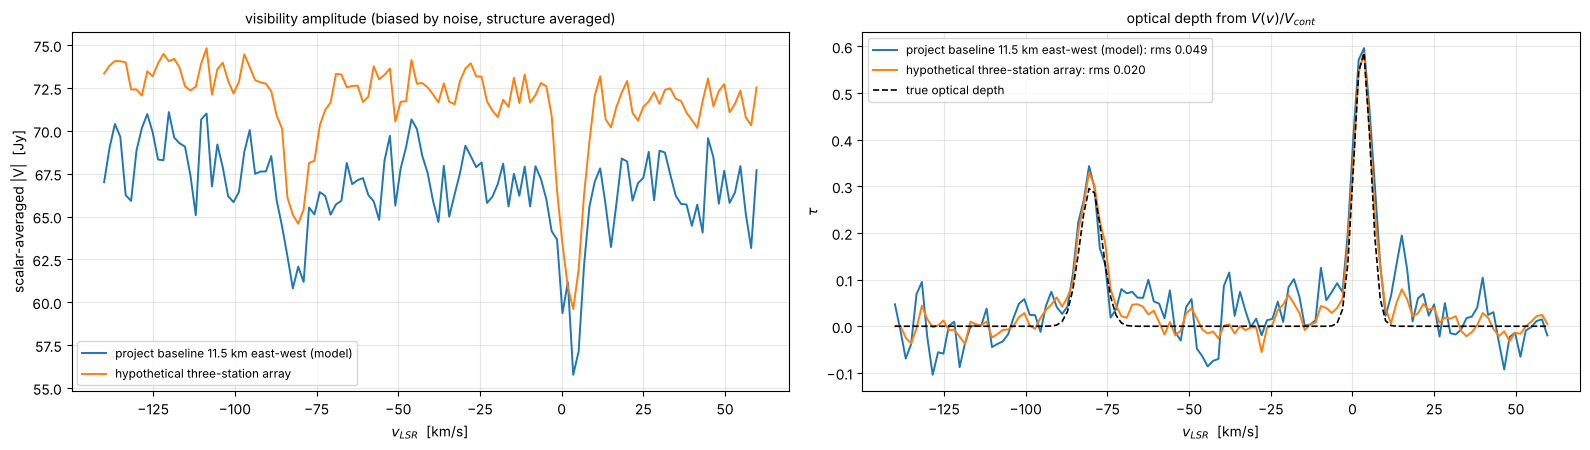
\includegraphics[width=\textwidth]{images/lines_hi_absorption.png}
  \caption{Cygnus~A at 21\,cm: scalar-averaged visibility amplitude and the
           optical depth from the line-to-continuum ratio.}
  \label{fig:lines-hi}
\end{figure}

\paragraph*{Integration time.} For S/N 5 per 977\,Hz channel on two 3\,m dishes
M1 needs 4.8\,h, a 20\,Jy maser 60\,h; the time falls with the fourth power of
the dish diameter (two 7.5\,m dishes: 6\,min). With the B210 at 2\,MS/s such
channels need an FFT length of 2048 or a decimated recording.
